\documentclass[professionalfont]{beamer}

\usepackage{graphicx}
\usepackage{newtxtext,newtxmath}
\usetheme{default}
\usecolortheme{seagull}

\setbeamertemplate{navigation symbols}{}
\setbeamertemplate{itemize item}{\textbullet} 
\setbeamertemplate{title page}{
    \begin{center}
        {\textcolor{blue}{\textbf{\fontsize{11}{14}\selectfont GSM-PLUS: A Comprehensive Benchmark for Evaluating the Robustness of LLMs as Mathematical Problem Solvers}}} \\[1.5cm]
        
        {\fontsize{9}{14}\selectfont Qintong Li, et al \\[0.3cm]
        The University of Hong Kong \& Tencent AI Lab \\[0.3cm]
        July 2, 2024}
    \end{center}
}
% ------------------ Title ------------------

\begin{document}
\frame{\titlepage}


\begin{frame}
\begin{center}
    { \textbf{\textcolor{blue}{ {\fontsize{12}{14}\selectfont Abstract} }} }
\end{center}

{\fontsize{10}{14}\selectfont 
\begin{itemize}
    \item Does LLM truly understand math, or simulate understanding?
    
    - Even slight variations in problem can lead to confusion for LLMs.
    
    - Enhancing the robustness of LLMs is essential.
\end{itemize}

\begin{itemize}
    \item We propose GSM-PLUS, which is more challenging than GSM-8K.
    
    - Highlighting the weaknesses of LLMs
    
    - Identifying solutions to address these weaknesses
\end{itemize}
}

\begin{center}
    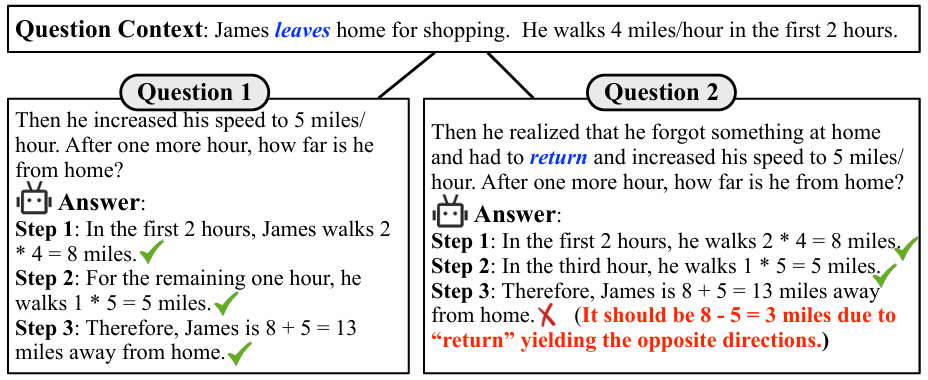
\includegraphics[width=0.8\textwidth]{figure1.png}
\end{center}
\end{frame}
% ------------------ Slide 1 ------------------

\begin{frame}
\begin{center}
    { \textbf{\textcolor{blue}{ {\fontsize{12}{14}\selectfont Introduction} }} }
\end{center}

{\fontsize{10}{14}\selectfont 
\begin{itemize}
    \item GSM-PLUS is 5 perturbations of GSM-8K
    
    - Numerical Variation
    
    - Arithmetic Variation
    
    - Problem understanding
    
    - Distractor insertion
    
    - Critical thinking
\end{itemize}

\begin{itemize}
    \item With perturbation, there is no difference in difficulty
    
    - Human performance is unaffected
    
    - LLMs showed a gap up to 20\% in accuracy
\end{itemize}
}

\end{frame}
% ------------------ Slide 2 ------------------

\begin{frame}
\begin{center}
    { \textbf{\textcolor{blue}{ {\fontsize{12}{14}\selectfont Perturbation Category} }} }
\end{center}

\begin{center}
    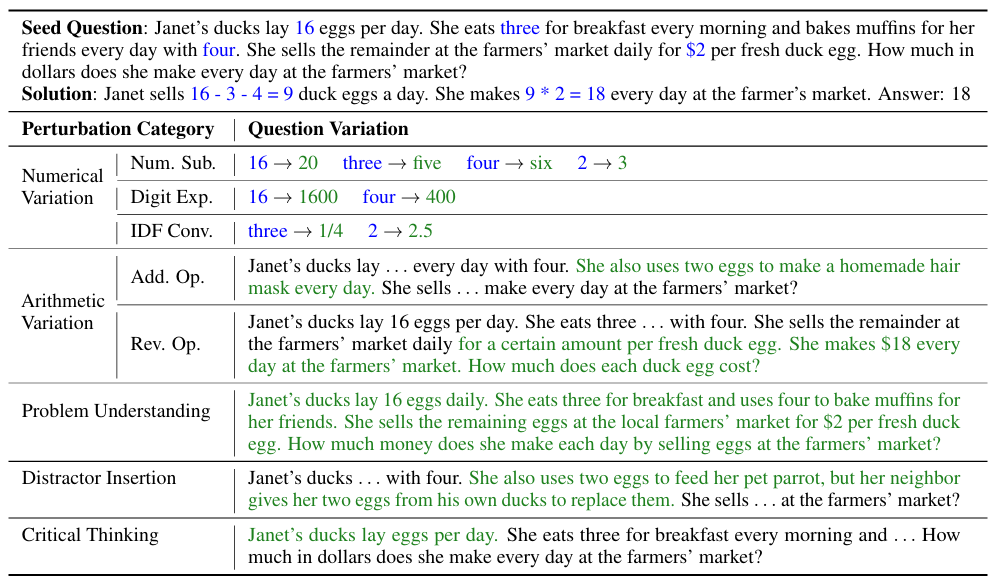
\includegraphics[width=1.0\textwidth]{table2.png}
\end{center}

\end{frame}
% ------------------ Slide 3 ------------------

\begin{frame}
\begin{center}
    { \textbf{\textcolor{blue}{ {\fontsize{12}{14}\selectfont Experiment} }} }
\end{center}

{\fontsize{10}{14}\selectfont 
\begin{itemize}
    \item Experimental Setup
    
    - Test for models like GPT-4, LLaMA-2, CodeLlama, etc.
    
    - Compare results in GSM-8K and GSM-PLUS

    - Observe Performance Drop Rate (PDR)
\end{itemize}

\begin{itemize}
    \item Overall Results
    
    - Quite robust to Numerical Variation, Problem understanding
    
    - Vulnerable to other variations
\end{itemize}
}

\begin{center}
    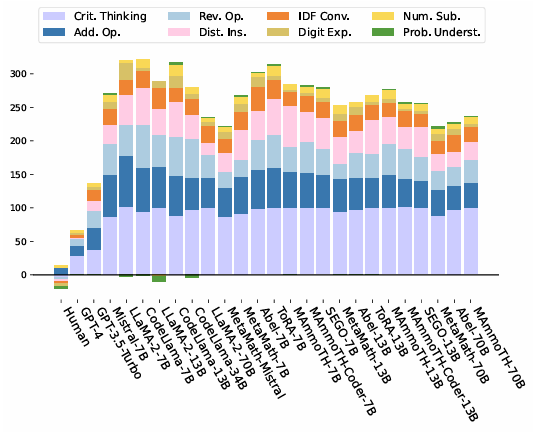
\includegraphics[width=0.5\textwidth]{figure2.png}
\end{center}

\end{frame}
% ------------------ Slide 4 ------------------

\begin{frame}
\begin{center}
    { \textbf{\textcolor{blue}{ {\fontsize{12}{14}\selectfont Solution for Robustness} }} }
\end{center}

{\fontsize{10}{14}\selectfont 
\begin{itemize}
    \item Compositional Prompting
    
    - Iteratively decompose complex problems
\end{itemize}
}

\begin{center}
    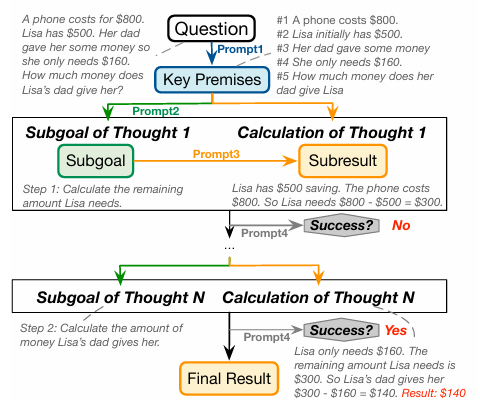
\includegraphics[width=0.7\textwidth]{figure5.png}
\end{center}

\end{frame}
% ------------------ Slide 5 ------------------

\begin{frame}
\begin{center}
    { \textbf{\textcolor{blue}{ {\fontsize{12}{14}\selectfont Conclusion} }} }
\end{center}
\\[0.5cm]

{\fontsize{10}{14}\selectfont 
\begin{itemize}
    \item Most LLMs showed large PDR in GSM-PLUS
    
    - Models need to be robust to minor variations
    
    - Compositional Prompting partially solved the problem
\end{itemize}
\\[0.5cm]
\begin{itemize}
    \item Limitation
    
    - Training over elementary school level is required.
    
    - Only accuracy of the answer, not the solution chain.

    - We don't know underlying reason of LLMs' failure.
\end{itemize}
}

\end{frame}
% ------------------ Slide 6 ------------------


\end{document}
